\begin{surferPage}[D4+-]{A $D_4^{+-}$ Singularity}
The following equation corresponds to the so-called $D_4^{+-}$-singularity:
    \vspace*{-0.4em}
    \begin{center}
      $x^2y+y^3-z^2=0.$
    \end{center}
    \vspace*{-0.4em}
    This is the surface variant of a plane singularity which 
    is a point in which three distinct straight lines meet,
but where two of those cannot be seen in the real word, but only in
a space with complex numbers.
    We get these three lines back from the surface equation when
    plugging $z=0$ into the equation.
    This yields the plane curve with equation $x^2y+y^3=0$ which is
    equivalent to three straight lines, but two non-real: $y\cdot(x-iy)\cdot(x+iy)=0$.
    \vspace*{-0.7em}
    \begin{center}
      \begin{tabular}{c@{\ }c@{\ }c@{\ }c}
        \begin{tabular}{@{}c@{}}
          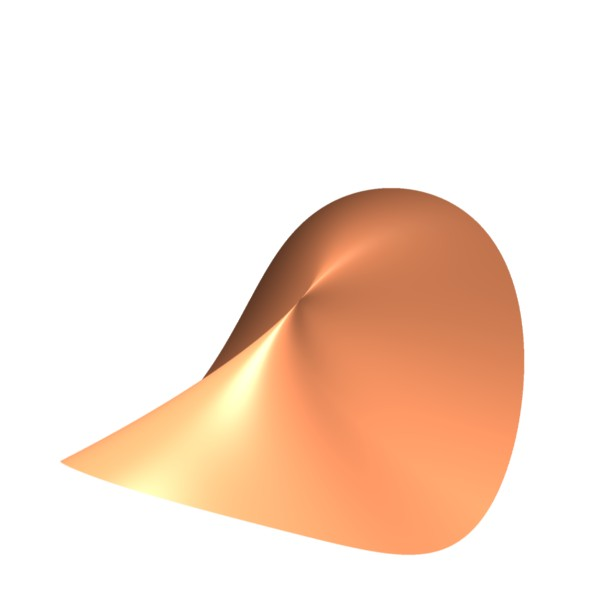
\includegraphics[width=1.2cm]{../../common/images/D4pm}
        \end{tabular}
        &
        \begin{tabular}{@{}c@{}}
          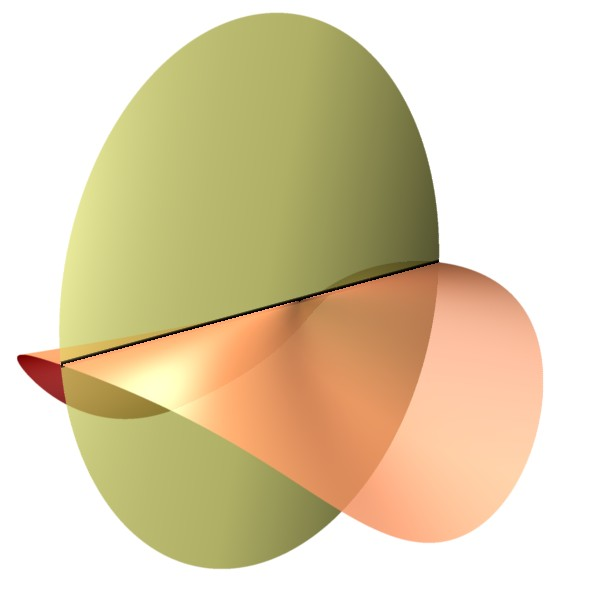
\includegraphics[width=1.2cm]{../../common/images/D4pm_def_with_plane_cut_0}
        \end{tabular}
     \end{tabular}
    \end{center}
    \vspace*{-0.4em}

It is difficult to visualize the geometry of this singularity in our
real world because an essential part only lives in the complex world. 
One attempt is to take the following deformation where for $a=0$ and
$b=0$ we get the original equation:
\[(y+a)\cdot(x^2+y^2)+by^2-z^2=0.\]
   \vspace*{-2em}
    \begin{center}
      \begin{tabular}{@{}c@{\quad}c@{\quad}c@{}}
        \begin{tabular}{@{}c@{}}
          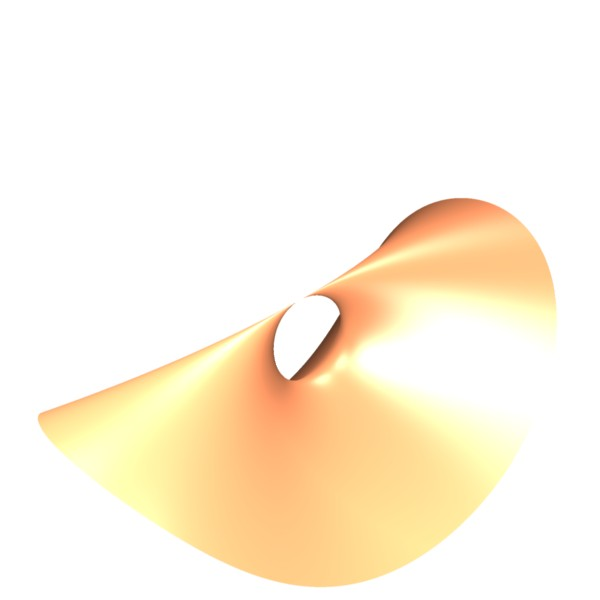
\includegraphics[width=1.1cm]{../../common/images/D4pm_1}
        \end{tabular}
        &
        \begin{tabular}{@{}c@{}}
          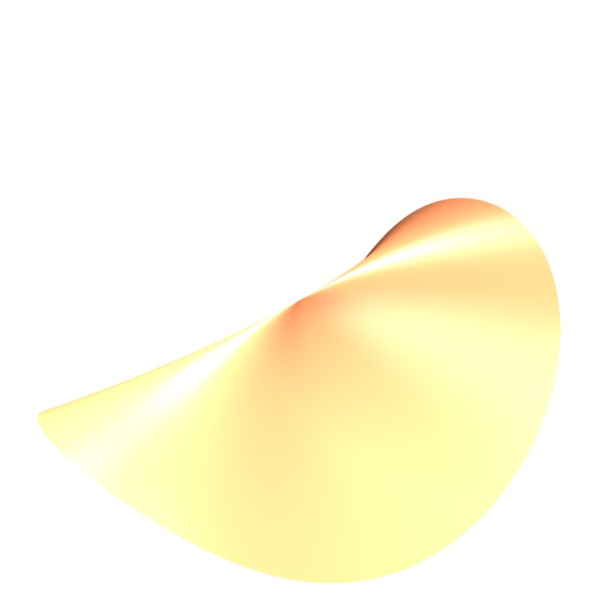
\includegraphics[width=1.1cm]{../../common/images/D4pm_0}
        \end{tabular}
        &
        \begin{tabular}{@{}c@{}}
          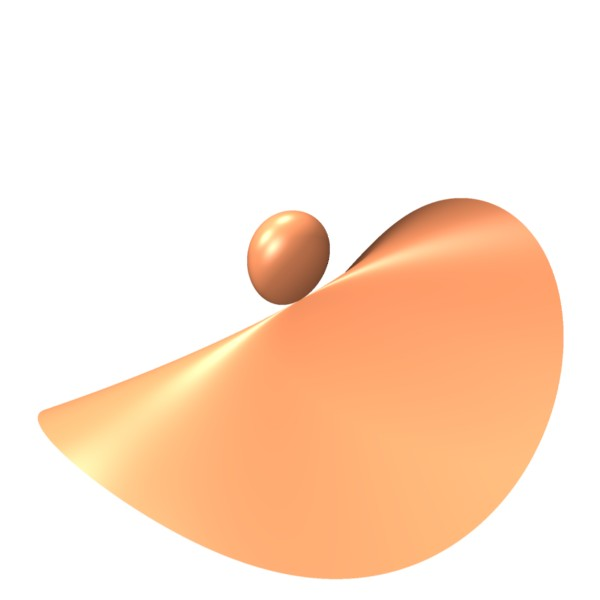
\includegraphics[width=1.1cm]{../../common/images/D4pm_2}
        \end{tabular}
\\
$b=-0.5$
& 
$b=0$
&
$b=0.5$
      \end{tabular}
    \end{center}
 
\end{surferPage}
